\documentclass{article}
\usepackage[utf8]{inputenc}
\usepackage{listings}
\usepackage{xcolor}
\usepackage{graphicx}
\usepackage{amsmath}
\usepackage{hyperref}

% Definir colores para el resaltado de sintaxis
\definecolor{codegreen}{rgb}{0,0.6,0}
\definecolor{codegray}{rgb}{0.5,0.5,0.5}
\definecolor{codepurple}{rgb}{0.58,0,0.82}
\definecolor{backcolour}{rgb}{0.95,0.95,0.92}

% Configuración para el código JavaScript
\lstdefinestyle{mystyle}{
    backgroundcolor=\color{backcolour},
    commentstyle=\color{codegreen},
    keywordstyle=\color{magenta},
    numberstyle=\tiny\color{codegray},
    stringstyle=\color{codepurple},
    basicstyle=\footnotesize,
    breakatwhitespace=false,
    breaklines=true,
    captionpos=b,
    keepspaces=true,
    numbers=left,
    numbersep=5pt,
    showspaces=false,
    showstringspaces=false,
    showtabs=false,
    tabsize=2
}

% Configuración para el lenguaje JavaScript
\lstset{style=mystyle, language=JavaScript}


\title{Métricas de Defectos en el Desarrollo de Software}
\author{Paul Wenceslao Condori Garcia}

\begin{document}

\maketitle

\section{Métricas de Defectos}

Las métricas de defectos en el desarrollo de software son herramientas esenciales para evaluar la calidad y la fiabilidad del código, así como para guiar el proceso de desarrollo y mantenimiento. Estas métricas proporcionan una visión cuantitativa de la presencia de defectos en el software, lo que permite a los equipos de desarrollo identificar áreas problemáticas, asignar recursos de manera efectiva y mejorar continuamente el proceso de desarrollo.

Las pruebas de software se consideran una tarea importante en el proceso de desarrollo de software, en el que el objetivo principal es encontrar errores o defectos. De hecho, teniendo en cuenta el gran volumen de casos de prueba necesarios para garantizar la calidad, los archivos más propensos a errores serían más prioritarios en la práctica.

\begin{figure}
  \centering
  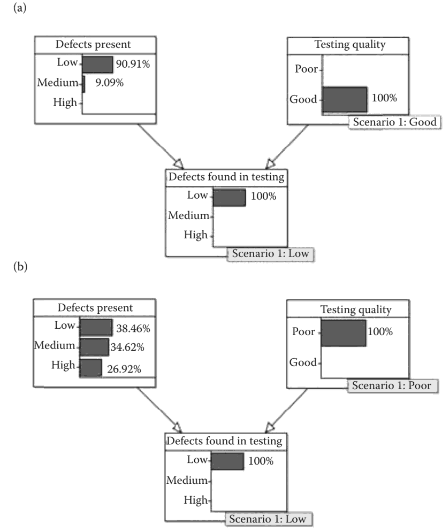
\includegraphics{md1.png}
  \label{fig:imagen}
\end{figure}


\section{Tipos Principales de Métricas de Defectos}

\begin{itemize}
    \item Tasa de Defectos: Esta métrica calcula la cantidad de defectos encontrados por unidad de medida, como por ejemplo, la cantidad de defectos por línea de código, por función, por componente, etc.
    
    \item Gravedad de los Defectos: Clasifica los defectos según su impacto en el software, desde defectos menores que tienen poco impacto en la funcionalidad hasta defectos críticos que pueden causar fallos importantes en el sistema.
    \item Tasa de Resolución de Defectos: Indica la velocidad con la que se corrigen los defectos después de ser identificados, lo que proporciona información sobre la eficiencia del proceso de desarrollo y prueba.
    \item Densidad de Defectos por Módulo: Evalúa la distribución de defectos en diferentes partes del software, lo que puede ayudar a identificar áreas problemáticas que requieren una mayor atención y pruebas adicionales.
\end{itemize}
\section{Tipos Principales de Métricas de Defectos}

\subsection{Tasa de Defectos (Defect Density)}
Esta métrica calcula la cantidad de defectos encontrados por unidad de medida, como por ejemplo, defectos por mil líneas de código (KLOC), por función, o por componente.

\begin{equation}
  \text{Tasa de Defectos} = \frac{\text{Número total de defectos}}{\text{Tamaño del software (en KLOC, funciones, etc.)}}
\end{equation}

\subsection{Gravedad de los Defectos (Defect Severity)}
Clasifica los defectos según su impacto en el software, desde defectos menores con poco impacto en la funcionalidad hasta defectos críticos que pueden causar fallos importantes en el sistema.

\subsubsection{Clasificaciones comunes}
\begin{itemize}
  \item \textbf{Crítico:} Defectos que causan fallos del sistema o pérdida de datos.
  \item \textbf{Alto:} Defectos que afectan significativamente la funcionalidad principal.
  \item \textbf{Medio:} Defectos que afectan la funcionalidad secundaria.
  \item \textbf{Bajo:} Defectos menores que no afectan significativamente la funcionalidad.
\end{itemize}

\subsection{Tasa de Resolución de Defectos (Defect Resolution Rate)}
Indica la velocidad con la que se corrigen los defectos después de ser identificados.

\begin{equation}
  \text{Tasa de Resolución de Defectos} = \frac{\text{Número de defectos corregidos}}{\text{Tiempo total para corregirlos}}
\end{equation}

\subsection{Densidad de Defectos por Módulo (Defect Density per Module)}
Evalúa la distribución de defectos en diferentes partes del software, lo que puede ayudar a identificar áreas problemáticas que requieren mayor atención y pruebas adicionales.

\begin{equation}
  \text{Densidad de Defectos por Módulo} = \frac{\text{Número de defectos en el módulo}}{\text{Tamaño del módulo (en KLOC, funciones, etc.)}}
\end{equation}

\subsection{Tasa de Introducción de Defectos (Defect Introduction Rate)}
Mide la cantidad de defectos introducidos durante un período específico, como por sprint, por mes, etc.

\begin{equation}
  \text{Tasa de Introducción de Defectos} = \frac{\text{Número de defectos introducidos}}{\text{Tiempo}}
\end{equation}


\section{Aplicaciones y Limitaciones}

Las métricas de defectos se utilizan para una variedad de propósitos en el desarrollo de software, incluyendo la evaluación de la calidad del software, la estimación de costos y tiempo de desarrollo, y el seguimiento del progreso del proyecto. 

%\subsection{Ejemplo de Código en JavaScript para Métricas de Defectos}


Sin embargo, estas métricas tienen ciertas limitaciones, ya que no proporcionan una indicación directa de la complejidad del código o de la calidad del software. Además, pueden fomentar un enfoque excesivo en la corrección de defectos en lugar de abordar las causas subyacentes de los mismos.

\section{Conclusiones}

A pesar de sus limitaciones, las métricas de defectos siguen siendo una herramienta valiosa para evaluar y mejorar la calidad del software. Se recomienda complementar estas métricas con otras medidas de calidad y complejidad del código para obtener una evaluación más completa del software. Al integrar métricas de defectos en el proceso de desarrollo de software, los equipos pueden identificar y abordar proactivamente los problemas de calidad, lo que conduce a un software más confiable y robusto

\section{Referencias}

\begin{itemize}
    \item Fenton, N., \& Pfleeger, S. L. (1998). Software Metrics: A Rigorous and Practical Approach. PWS Publishing Co.
    \item Kan, S. H. (2002). Metrics and Models in Software Quality Engineering. Addison-Wesley.
    \item Öztürk, M. M. (2017). Which type of metrics are useful to deal with class imbalance in software defect prediction? Information and Software Technology, 92, 17-29.
    \item Shiri Harzevili, N., \& Alizadeh, S. H. (2021). Analysis and modeling conditional mutual dependency of metrics in software defect prediction using latent variables. Neurocomputing, 460.
\end{itemize}

\end{document}
